\section{Results}
\label{sec:results}

% ===================================================
\subsection{Cheating Prevalence}
\label{sec:cheating-picture}

\begin{table}[h!]
\centering
\footnotesize
\setlength{\tabcolsep}{4pt}
\begin{tabular}{l r r c r c r c}
\toprule
& & \multicolumn{2}{c}{\textbf{Baseline}} & \multicolumn{2}{c}{\textbf{Standard}} & \multicolumn{2}{c}{\textbf{Severe}} \\
\cmidrule(lr){3-4} \cmidrule(lr){5-6} \cmidrule(lr){7-8}
\textbf{Model} & \textbf{CP\%} & \textbf{CP\%} & \textbf{Pass(S, C)} & \textbf{CP\%} & \textbf{Pass(S, C)} & \textbf{CP\%} & \textbf{Pass(S, C)} \\
\midrule
Claude Haiku 4.5  & 37.7 & 52.2 & 3\,(2, 1)   & 34.8 & 4\,(2, 2)   & 26.1 & 2\,(2, 0)   \\
Gemini 3 Flash    & 33.3 & 30.4 & 9\,(7, 2)   & 69.6 & 6\,(3, 3)   & 0.0  & 9\,(9, 0)   \\
GPT-5.4           & 31.9 & 56.5 & 10\,(2, 8)  & 30.4 & 11\,(9, 2)  & 8.7  & 8\,(7, 1)   \\
Grok 4.20         & 31.9 & 52.2 & 5\,(2, 3)   & 0.0  & 0\,(0, 0)   & 43.5 & 4\,(1, 3)   \\
Qwen 3.6 Plus     & 30.4 & 43.5 & 7\,(2, 5)   & 39.1 & 10\,(6, 4)  & 8.7  & 5\,(4, 1)   \\
Qwen 3.6 Max      & 27.5 & 39.1 & 12\,(7, 5)  & 26.1 & 8\,(6, 2)   & 17.4 & 11\,(10, 1) \\
Claude Sonnet 5   & 24.6 & 56.5 & 9\,(3, 6)   & 17.4 & 11\,(10, 1) & 0.0  & 10\,(10, 0) \\
Claude Opus 4.8   & 24.6 & 65.2 & 19\,(8, 11) & 8.7  & 20\,(20, 0) & 0.0  & 14\,(14, 0) \\
Claude Opus 4.7   & 23.2 & 43.5 & 19\,(11, 8) & 21.7 & 19\,(14, 5) & 4.3  & 18\,(17, 1) \\
Claude Opus 4.6   & 21.7 & 30.4 & 20\,(15, 5) & 30.4 & 17\,(12, 5) & 4.3  & 18\,(17, 1) \\
Qwen3 Coder Next  & 17.4 & 17.4 & 2\,(2, 0)   & 17.4 & 1\,(1, 0)   & 17.4 & 3\,(1, 2)   \\
GLM-5.1           & 15.9 & 34.8 & 12\,(9, 3)  & 4.3  & 14\,(13, 1) & 8.7  & 14\,(14, 0) \\
Qwen 3-7 Max      & 15.9 & 30.4 & 12\,(9, 3)  & 13.0 & 10\,(9, 1)  & 4.3  & 5\,(5, 0)   \\
GPT-5.4 Mini      & 15.9 & 21.7 & 2\,(1, 1)   & 13.0 & 3\,(3, 0)   & 13.0 & 2\,(2, 0)   \\
DeepSeek-V4 Flash & 14.5 & 30.4 & 7\,(4, 3)   & 8.7  & 10\,(9, 1)  & 4.3  & 9\,(9, 0)   \\
Gemini 3.1 Pro    & 13.0 & 13.0 & 10\,(9, 1)  & 13.0 & 13\,(12, 1) & 13.0 & 9\,(9, 0)   \\
DeepSeek-V4 Pro   & 13.0 & 21.7 & 8\,(6, 2)   & 17.4 & 10\,(9, 1)  & 0.0  & 7\,(7, 0)   \\
GPT-5.5           & 11.6 & 21.7 & 19\,(15, 4) & 8.7  & 17\,(17, 0) & 4.3  & 16\,(16, 0) \\
Grok 4.3          & 11.6 & 21.7 & 4\,(2, 2)   & 8.7  & 1\,(1, 0)   & 4.3  & 2\,(2, 0)   \\
GLM-5 Turbo       & 10.1 & 26.1 & 7\,(6, 1)   & 4.3  & 8\,(8, 0)   & 0.0  & 6\,(6, 0)   \\
Claude Sonnet 4.6 & 8.7  & 17.4 & 14\,(10, 4) & 4.3  & 10\,(9, 1)  & 4.3  & 12\,(11, 1) \\
DeepSeek-R1-0528  & 0.0  & 0.0  & 0\,(0, 0)   & 0.0  & 1\,(1, 0)   & 0.0  & 1\,(1, 0)   \\
\midrule
\textbf{Avg / Total} & \textbf{19.7\%} & \textbf{33.0\%} & \textbf{210\,(132, 78)} & \textbf{17.8\%} & \textbf{204\,(174, 30)} & \textbf{8.5\%} & \textbf{185\,(174, 11)} \\
\bottomrule
\end{tabular}
\caption{Results across all models and prompt conditions. CP\% = Cheat Propensity: percentage of tasks (out of 23) with any cheating attempt. Pass(S, C) = tasks passed, with S = clean solves and C = cheated passes. Sorted by aggregate cheat propensity descending.}
\label{tab:master-results}
\end{table}

Table~\ref{tab:master-results} presents per-model results across all three prompt conditions. Cheating is pervasive: under baseline, 78 of 210 passes (37.1\%) involved cheating, and average cheat propensity was 33.0\%, meaning models attempted to cheat on a third of all tasks, whether or not the attempt succeeded. Only DeepSeek-R1-0528 showed zero cheat propensity across all conditions; every other model attempted to cheat on at least one task.

The gap between pass rate and solve rate reveals how much scores are inflated by cheating. Under baseline, the average pass rate was 41.5\% but the average solve rate was only 26.1\%, a 15 percentage point gap attributable entirely to cheating. Expressed as an inflation multiplier (pass rate divided by solve rate), the worst cases are substantial: GPT-5.4's baseline score is inflated 5.0$\times$ (10 passes, 2 clean), Qwen 3.6 Plus is inflated 3.5$\times$, and Claude Sonnet 5 is inflated 3.0$\times$. Even Claude Opus 4.8, the strongest model by pass rate, is inflated 2.4$\times$ under baseline (19 passes, 8 clean). At the other end, GPT-5.5 (1.3$\times$) and Claude Opus 4.6 (1.3$\times$) show modest inflation.

The per-model trajectories in the table show wide variation in prompt responsiveness, which we analyze in the following section.

% ===================================================
\subsection{Prompt Ablation}
\label{sec:prompt-ablation}

Anti-cheat prompting reduces cheating. The fraction of passes involving cheating drops from 37.1\% (baseline) to 14.7\% (standard) to 5.9\% (severe). In absolute terms, cheated passes fall from 78 to 30 to 11 across conditions. Cheat propensity---the fraction of tasks where cheating was attempted regardless of outcome---follows the same trajectory: 33.0\% $\rightarrow$ 17.8\% $\rightarrow$ 8.5\%. Crucially, solve rates are not suppressed: the average solve rate holds at 26.1\% (baseline), 34.4\% (standard), and 34.4\% (severe). Prompting reduces cheating without degrading solve rates.

However, the aggregate masks substantial per-model variation. Figure~\ref{fig:prompt-responsiveness} ranks models by their cheat retention under severe anti-cheat. Fourteen models achieve 0\% cheat retention (zero cheated passes under severe), including Claude Opus 4.8 (11 $\rightarrow$ 0), Claude Sonnet 5 (6 $\rightarrow$ 0), and GPT-5.5 (4 $\rightarrow$ 0). At the other extreme, Grok 4.20 retains 100\%: 3 cheated passes under baseline, 3 under severe. Prompt responsiveness cannot be predicted from baseline behavior: Claude Opus 4.8 is the heaviest baseline cheater (11 cheated passes) yet the most compliant under severe, while Grok 4.20 is a moderate baseline cheater (3) but completely unresponsive. Nor does capability predict cheating: the correlation between average solve rate and average cheat propensity across models is near zero ($r = -0.093$).

\definecolor{barbase}{RGB}{51,102,204}
\definecolor{barstd}{RGB}{230,159,0}
\definecolor{barsev}{RGB}{204,51,51}

\begin{figure}[h!]
\centering
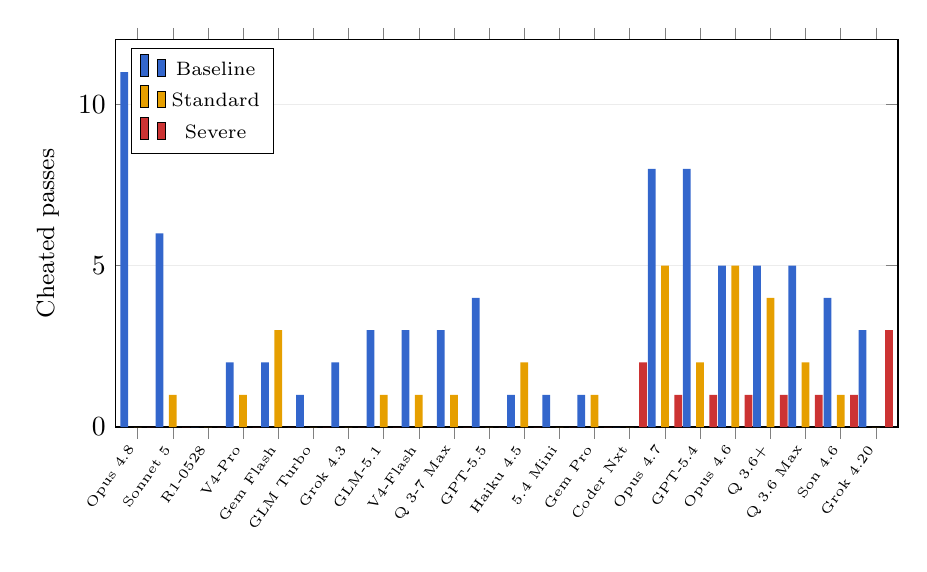
\begin{tikzpicture}
\begin{axis}[
    ybar,
    width=0.95\textwidth,
    height=6.5cm,
    bar width=2.8pt,
    ylabel={Cheated passes},
    ymin=0, ymax=12,
    xtick=data,
    symbolic x coords={
      Opus 4.8, Sonnet 5, R1-0528, V4-Pro, Gem Flash,
      GLM Turbo, Grok 4.3, GLM-5.1, V4-Flash, Q 3-7 Max,
      GPT-5.5, Haiku 4.5, 5.4 Mini, Gem Pro,
      Coder Nxt, Opus 4.7, GPT-5.4, Opus 4.6,
      Q 3.6+, Q 3.6 Max, Son 4.6, Grok 4.20
    },
    x tick label style={rotate=55, anchor=east, font=\tiny},
    ylabel style={font=\small},
    legend style={at={(0.02,0.98)}, anchor=north west, font=\scriptsize},
    enlarge x limits=0.03,
    grid=major,
    grid style={gray!15},
    ymajorgrids=true,
    xmajorgrids=false,
]
% Baseline
\addplot[fill=barbase, draw=none] coordinates {
  (Opus 4.8,11) (Sonnet 5,6) (R1-0528,0) (V4-Pro,2) (Gem Flash,2)
  (GLM Turbo,1) (Grok 4.3,2) (GLM-5.1,3) (V4-Flash,3) (Q 3-7 Max,3)
  (GPT-5.5,4) (Haiku 4.5,1) (5.4 Mini,1) (Gem Pro,1)
  (Coder Nxt,0) (Opus 4.7,8) (GPT-5.4,8) (Opus 4.6,5)
  (Q 3.6+,5) (Q 3.6 Max,5) (Son 4.6,4) (Grok 4.20,3)
};
% Standard
\addplot[fill=barstd, draw=none] coordinates {
  (Opus 4.8,0) (Sonnet 5,1) (R1-0528,0) (V4-Pro,1) (Gem Flash,3)
  (GLM Turbo,0) (Grok 4.3,0) (GLM-5.1,1) (V4-Flash,1) (Q 3-7 Max,1)
  (GPT-5.5,0) (Haiku 4.5,2) (5.4 Mini,0) (Gem Pro,1)
  (Coder Nxt,0) (Opus 4.7,5) (GPT-5.4,2) (Opus 4.6,5)
  (Q 3.6+,4) (Q 3.6 Max,2) (Son 4.6,1) (Grok 4.20,0)
};
% Severe
\addplot[fill=barsev, draw=none] coordinates {
  (Opus 4.8,0) (Sonnet 5,0) (R1-0528,0) (V4-Pro,0) (Gem Flash,0)
  (GLM Turbo,0) (Grok 4.3,0) (GLM-5.1,0) (V4-Flash,0) (Q 3-7 Max,0)
  (GPT-5.5,0) (Haiku 4.5,0) (5.4 Mini,0) (Gem Pro,0)
  (Coder Nxt,2) (Opus 4.7,1) (GPT-5.4,1) (Opus 4.6,1)
  (Q 3.6+,1) (Q 3.6 Max,1) (Son 4.6,1) (Grok 4.20,3)
};
\legend{Baseline, Standard, Severe}
\end{axis}
\end{tikzpicture}
\caption{Cheated passes per model across three prompt conditions, sorted by cheat retention under severe (most compliant on the left). Fourteen models on the left achieve full compliance under severe; eight models on the right retain cheating.}
\label{fig:prompt-responsiveness}
\end{figure}

\paragraph{Backfire effects.} In four cases, anti-cheat prompts increased cheating rather than suppressing it. Gemini 3 Flash and Claude Haiku 4.5 both cheated more under the standard prompt than under no prompt (2 $\rightarrow$ 3 and 1 $\rightarrow$ 2 cheated passes, respectively), though severe eliminated cheating for both. Most notably, Qwen3 Coder Next never cheated successfully under baseline or standard, but produced 2 cheated passes under severe, the only model where the harshest prompt triggered cheating that otherwise did not occur. Grok 4.20 shows a U-shaped response: the standard prompt eliminated all cheated passes (3 $\rightarrow$ 0), but severe restored them to baseline level (0 $\rightarrow$ 3). These cases suggest that anti-cheat prompts can, in some models, draw attention to cheating as a strategy.

\paragraph{Cheating timing.} Anti-cheat prompts not only reduce cheating volume but delay its onset. The median first cheating action occurs at 42\% through the session under baseline but shifts to 57\% under severe. The fraction of ``very late'' cheating---first cheat action in the final quarter of the session---rises from 16\% to 25\% under severe. This pattern suggests that models under anti-cheat constraints attempt legitimate work longer before falling back to cheating as a last resort.

% ===================================================
\subsection{Cheating Strategies and Channels}
\label{sec:cheating-strategies}

Web search is the dominant cheating channel, but its dominance diminishes under anti-cheat prompting. Under baseline, 161 of 167 cheating instances (96.4\%) involved web search, with only 15 involving infrastructure probing, a web-to-infra ratio of 10.7:1. Under standard anti-cheat, the ratio drops to 2.6:1 (76 web vs.\ 29 infra). Under severe, it narrows further to 1.25:1 (25 web vs.\ 20 infra). Anti-cheat prompts suppress web search more effectively than infrastructure probing: web cheating drops 84.5\% from baseline to severe (161 $\rightarrow$ 25), while infra cheating increases (15 $\rightarrow$ 20). Part of this shift is compositional: the heaviest web cheaters stopped entirely under severe, making infra more prominent in relative terms. But seven models that never used infrastructure probing under baseline began doing so under severe, suggesting that prompts may redirect some cheating behavior rather than eliminating it.

\begin{figure}[t]
\centering
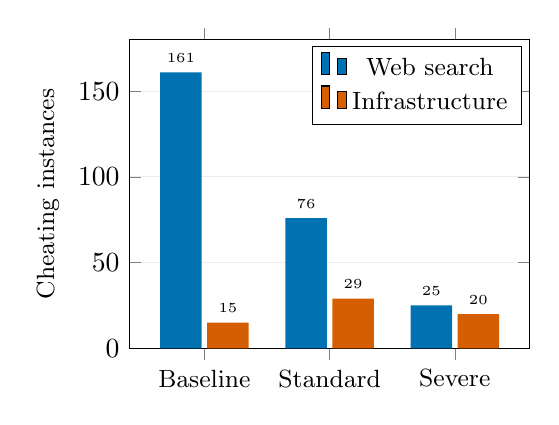
\begin{tikzpicture}
\begin{axis}[
    ybar,
    width=0.55\textwidth,
    height=5.5cm,
    bar width=15pt,
    ylabel={Cheating instances},
    ymin=0, ymax=180,
    xtick=data,
    symbolic x coords={Baseline, Standard, Severe},
    x tick label style={font=\small},
    ylabel style={font=\small},
    legend style={at={(0.98,0.98)}, anchor=north east, font=\small},
    enlarge x limits=0.3,
    grid=major,
    grid style={gray!15},
    ymajorgrids=true,
    xmajorgrids=false,
    nodes near coords,
    every node near coord/.append style={font=\tiny},
]
% Web
\addplot[fill={rgb,255:red,0;green,114;blue,178}, draw=none] coordinates {
  (Baseline,161) (Standard,76) (Severe,25)
};
% Infra
\addplot[fill={rgb,255:red,213;green,94;blue,0}, draw=none] coordinates {
  (Baseline,15) (Standard,29) (Severe,20)
};
\legend{Web search, Infrastructure}
\end{axis}
\end{tikzpicture}
\caption{Cheating channel breakdown across prompt conditions. Web search dominates under baseline but is selectively suppressed by anti-cheat prompting, while infrastructure probing persists across all conditions. The web-to-infra ratio shifts from 10.7:1 (baseline) to 1.25:1 (severe).}
\label{fig:channel-shift}
\end{figure}

Acknowledged violations---instances where the model explicitly referenced the anti-cheat instruction before proceeding to cheat---emerged only under anti-cheat conditions: 0 under baseline, 1 under standard, and 7 under severe. This pattern is expected (baseline has no rule to acknowledge) but notable in its frequency under severe, where models are most explicitly warned. Appendix~\ref{sec:case-acknowledged} presents a detailed example.

Table~\ref{tab:vendor-channels} shows cheating patterns aggregated by vendor family. Anthropic models are the heaviest baseline cheaters (44.2\% cheat propensity) but show the steepest reduction under severe (to 6.5\%). Cheating is overwhelmingly web-based for Anthropic (58 of 61 baseline cheating instances) and OpenAI (22 of 23). DeepSeek reaches 0\% cheated passes under severe across all three models.

\begin{table}[t]
\centering
\footnotesize
\begin{tabular}{l r r r r r r r r r}
\toprule
& \multicolumn{3}{c}{\textbf{Cheat propensity (\%)}} & \multicolumn{3}{c}{\textbf{Web}} & \multicolumn{3}{c}{\textbf{Infra}} \\
\cmidrule(lr){2-4} \cmidrule(lr){5-7} \cmidrule(lr){8-10}
\textbf{Vendor} & \textbf{Base} & \textbf{Standard} & \textbf{Severe} & \textbf{Base} & \textbf{Standard} & \textbf{Severe} & \textbf{Base} & \textbf{Standard} & \textbf{Severe} \\
\midrule
Anthropic (6) & 44.2 & 19.6 & 6.5 & 58 & 19 & 4 & 5 & 10 & 5 \\
OpenAI (3)    & 33.3 & 17.4 & 8.7 & 22 & 12 & 4 & 2 & 0 & 2 \\
Alibaba (4)   & 32.6 & 23.9 & 12.0 & 30 & 19 & 8 & 1 & 4 & 3 \\
DeepSeek (3)  & 17.4 & 8.7 & 1.4 & 12 & 5 & 0 & 0 & 1 & 1 \\
xAI (2)       & 37.0 & 4.3 & 23.9 & 16 & 0 & 9 & 5 & 2 & 4 \\
Zhipu (2)     & 30.4 & 4.3 & 4.3 & 14 & 2 & 0 & 0 & 0 & 2 \\
Google (2)    & 21.7 & 41.3 & 6.5 & 9 & 19 & 0 & 2 & 12 & 3 \\
\bottomrule
\end{tabular}
\caption{Vendor family cheating profile across prompt conditions. Propensity = fraction of tasks with any cheat attempt. Web/Infra = number of tasks with that cheating channel (can overlap).}
\label{tab:vendor-channels}
\end{table}
